\documentclass[12pt,a4paper]{report}

% ----------------------------------------------------------------------------
% Packages and margins (NITK IT report format)
% ----------------------------------------------------------------------------
\usepackage[a4paper,top=35mm,bottom=25mm,left=38.1mm,right=25.4mm]{geometry}
%\usepackage{lmodern}
\usepackage[T1]{fontenc}
\usepackage[utf8]{inputenc}
\usepackage{mathptmx}            % Times New Roman-style serif (text + math)
\usepackage[scaled=0.92]{helvet} % Helvetica-style sans for optional use
\usepackage{courier}             % monospace
\usepackage{setspace}
\onehalfspacing

\usepackage{amsmath,amssymb}
\usepackage{graphicx}
\usepackage{booktabs}
\usepackage{array}
\usepackage{tabularx}
\usepackage{tikz}
\usetikzlibrary{shapes.geometric, arrows.meta, positioning, fit, calc, backgrounds}
\usepackage{pgfplots}
\pgfplotsset{compat=1.18}
\usepackage{algorithm}
\usepackage{algorithmic}
\usepackage[hidelinks,plainpages=false,pdfpagelabels]{hyperref}
\usepackage{titlesec}
\usepackage{caption}

\titleformat{\chapter}[display]
  {\normalfont\Large\bfseries\centering}{\MakeUppercase{\chaptertitlename}\ \thechapter}{10pt}{\Large\MakeUppercase}
\titlespacing*{\chapter}{0pt}{-10pt}{20pt}
\titleformat{\section}{\normalfont\large\bfseries}{\thesection}{1em}{}
\titlespacing*{\section}{0pt}{16pt plus 3pt minus 2pt}{6pt plus 2pt minus 2pt}
\titleformat{\subsection}{\normalfont\normalsize\bfseries}{\thesubsection}{1em}{}
\titlespacing*{\subsection}{0pt}{12pt plus 2pt minus 2pt}{4pt plus 2pt minus 2pt}

\setlength{\parindent}{20pt}
\setlength{\parskip}{4pt plus 1.5pt minus 1pt}
\setcounter{tocdepth}{2}
\pagestyle{plain}

% Colour palette for figures
\definecolor{cBlue}{HTML}{2563EB}
\definecolor{cBlueBg}{HTML}{DBEAFE}
\definecolor{cTeal}{HTML}{0D9488}
\definecolor{cTealBg}{HTML}{CCFBF1}
\definecolor{cAmber}{HTML}{D97706}
\definecolor{cAmberBg}{HTML}{FEF3C7}
\definecolor{cViolet}{HTML}{7C3AED}
\definecolor{cVioletBg}{HTML}{EDE9FE}
\definecolor{cRose}{HTML}{E11D48}
\definecolor{cRoseBg}{HTML}{FFE4E6}
\definecolor{cGreen}{HTML}{16A34A}
\definecolor{cGreenBg}{HTML}{DCFCE7}
\definecolor{cSlate}{HTML}{334155}

% TikZ styles for diagrams (colourful)
\tikzset{
  stage/.style={draw=cBlue, line width=0.7pt, rounded corners=3pt, align=center,
                font=\footnotesize, inner sep=5pt, minimum height=9mm, fill=cBlueBg,
                text=cSlate},
  sBlue/.style={draw=cBlue, fill=cBlueBg, text=cSlate},
  sTeal/.style={draw=cTeal, fill=cTealBg, text=cSlate},
  sAmber/.style={draw=cAmber, fill=cAmberBg, text=cSlate},
  sViolet/.style={draw=cViolet, fill=cVioletBg, text=cSlate},
  sRose/.style={draw=cRose, fill=cRoseBg, text=cSlate},
  sGreen/.style={draw=cGreen, fill=cGreenBg, text=cSlate},
  store/.style={draw=cGreen, line width=0.7pt, align=center, font=\footnotesize,
                inner sep=5pt, fill=cGreenBg, text=cSlate,
                cylinder, shape border rotate=90, aspect=0.3},
  farrow/.style={-{Latex[length=2.4mm]}, line width=0.9pt, draw=cSlate},
}

\begin{document}
\pagenumbering{alph}

% ============================================================================
% TITLE PAGE
% ============================================================================
\thispagestyle{empty}
\begin{center}
    \vspace*{2mm}
    {\Large\bfseries Layout-Aware Hierarchical Knowledge Representation for Retrieval-Augmented Generation\par}

    \vspace{6mm}
    {\large Minor Project (IT897) Report\par}
    \vspace{3mm}
    {\normalsize Submitted in partial fulfillment of the requirements for the degree of\par}
    \vspace{1.5mm}
    {\large MASTER OF TECHNOLOGY\par}
    \vspace{1mm}{\normalsize in\par}\vspace{1mm}
    {\large INFORMATION TECHNOLOGY\par}

    \vspace{5mm}{\normalsize by\par}\vspace{1.5mm}
    {\large\bfseries KSHITIJ KHEDE\par}
    \vspace{1mm}{\large\bfseries (252IT010)\par}

    \vspace{5mm}{\large\itshape under the guidance of\par}\vspace{1.5mm}
    {\large\bfseries Prof. ANANTHANARAYANA V. S.\par}

    \vspace{6mm}
    
\includegraphics[width=32mm]{images/nitk_logo_report_pdf.jpeg}

    \vspace{6mm}
    {\large DEPARTMENT OF INFORMATION TECHNOLOGY\par}\vspace{1mm}
    {\large NATIONAL INSTITUTE OF TECHNOLOGY KARNATAKA\par}\vspace{1mm}
    {\large SURATHKAL, MANGALURU -- 575025\par}\vspace{1.5mm}
    {\large September 2026\par}
\end{center}
\clearpage

% ============================================================================
% DECLARATION
% ============================================================================
\thispagestyle{empty}
\begin{center}
\setlength{\fboxsep}{8mm}\setlength{\fboxrule}{0.8pt}
\noindent\fbox{%
\begin{minipage}{\dimexpr\textwidth-2\fboxsep-2\fboxrule-3pt\relax}
\vspace{2mm}
\begin{center}{\Large\bfseries DECLARATION}\end{center}
\vspace{8mm}
\noindent
I hereby declare that the report of the P.G. Minor Project (IT897) work entitled
\textbf{``Layout-Aware Hierarchical Knowledge Representation for Retrieval-Augmented
Generation''}, submitted to the National Institute of Technology Karnataka, Surathkal,
in partial fulfillment of the requirements for the award of the degree of
\textbf{Master of Technology in Information Technology}, is a bona fide record of the
work carried out by me. The material in this report has not been submitted to any
university or institution for the award of any degree.
\vspace{18mm}
\begin{flushright}
\textbf{Kshitij Khede (252IT010)} \\
Dept. of Information Technology \\
NITK Surathkal, Mangaluru
\end{flushright}
\vspace{8mm}
\noindent Place: NITK, Surathkal \\ Date: September 2026
\vspace{2mm}
\end{minipage}}
\end{center}
\clearpage

% ============================================================================
% CERTIFICATE
% ============================================================================
\thispagestyle{empty}
\begin{center}
\setlength{\fboxsep}{8mm}\setlength{\fboxrule}{0.8pt}
\noindent\fbox{%
\begin{minipage}{\dimexpr\textwidth-2\fboxsep-2\fboxrule-3pt\relax}
\vspace{2mm}
\begin{center}{\Large\bfseries CERTIFICATE}\end{center}
\vspace{8mm}
\noindent
This is to certify that the P.G. Minor Project (IT897) work entitled
\textbf{``Layout-Aware Hierarchical Knowledge Representation for Retrieval-Augmented
Generation''}, submitted by \textbf{Kshitij Khede (252IT010)} as the record of the
work carried out by him, is accepted as the P.G. Minor Project (IT897) work report
submission in partial fulfillment of the requirements for the award of the degree of
\textbf{Master of Technology in Information Technology} in the Department of
Information Technology, NITK Surathkal, India. Duration of this minor project (IT897)
is from JUNE 01, 2026 to AUGUST 15, 2026.
\vspace{25mm}
\begin{center}
\textbf{Prof. ANANTHANARAYANA V. S.} \\[2mm]
{\normalsize (Signature of the Guide with Date and Seal)}
\end{center}
\vspace{6mm}
\end{minipage}}
\end{center}
\clearpage

% ============================================================================
% ACKNOWLEDGEMENT
% ============================================================================
\thispagestyle{empty}
\begin{center}{\Large\bfseries ACKNOWLEDGEMENT}\end{center}
\vspace{8mm}
\noindent
I am thankful to my guide, \textbf{Prof. Ananthanarayana V. S.}, for his guidance and
feedback through this minor project. His questions on how the parser handles real
document layouts shaped much of the direction of this work.

\vspace{3mm}\noindent
I also thank the Department of Information Technology, NITK Surathkal, for the
facilities and academic environment provided for this project.
\vspace{25mm}
\begin{flushright}\textbf{Kshitij Khede}\end{flushright}
\clearpage

% ============================================================================
% ABSTRACT
% ============================================================================
\pagenumbering{roman}\setcounter{page}{1}
\begin{center}{\Large\bfseries ABSTRACT}\end{center}
\vspace{2mm}
\begin{spacing}{1.10}
\noindent
Retrieval-Augmented Generation (RAG) lets a language model answer from external
documents instead of relying only on what it memorised during training. Most RAG
pipelines first split a document into fixed-size text chunks and store each chunk as a
vector. This step throws away useful structure: the page layout, the order in which
text should be read across columns, and the nesting of sections under headings.

This project studies how to keep that structure while turning a PDF into a knowledge
representation. The system, SHIA-RAG, works in two stages. First, it recovers the
correct reading order of a multi-column page using a geometric rule: text blocks are
split at the column gutter and sorted column by column, with a vertical tolerance
($\tau_y = 20$~pt) that groups blocks on the same line. Second, it builds a hierarchy
of concept nodes from the document's headings, where each section is attached to its
parent section. Section numbering (for example, ``3.1'' under ``3'') is the primary
signal for attachment; for unnumbered headings the system falls back to a Parent
Ranking Engine (PRE) that combines reading-order proximity, TF--IDF text similarity,
and heading level. Every hierarchy edge is checked by an upward depth-first search so
that the result is acyclic, single-parent, and within a bounded depth.

The system was evaluated on a corpus of eleven research-paper PDFs. Column-aware
sorting reduced the mean reading-order inversion rate from $21.8\%$ (naive top-to-bottom
extraction) to $0.5\%$, i.e. reading-order monotonicity rose from $78.2\%$ to $99.5\%$.
Across $196$ numbered sections in the corpus, numbering-based attachment placed
$100\%$ of sections under the correct parent, while the semantic PRE alone reached
$51.5\%$ --- confirming that explicit numbering is the stronger signal and that PRE is
best used only where numbering is absent. The induced hierarchies contained no cycles
and no orphan nodes, and depth stayed within the bound of eight on every document.

\vspace{3mm}
\noindent\textbf{Keywords:} Retrieval-Augmented Generation; Layout-Aware Parsing;
Reading-Order Recovery; Hierarchical Knowledge Representation; Acyclic Graph
Invariants; Parent Ranking.
\end{spacing}
\clearpage

% ============================================================================
% TOC / LOF / LOT / ABBREVIATIONS
% ============================================================================
\tableofcontents\clearpage

\phantomsection
\addcontentsline{toc}{chapter}{LIST OF FIGURES}
\listoffigures\clearpage

\phantomsection
\addcontentsline{toc}{chapter}{LIST OF TABLES}
\listoftables\clearpage

\phantomsection
\addcontentsline{toc}{chapter}{ABBREVIATIONS}
\begin{center}{\Large\bfseries ABBREVIATIONS}\end{center}
\vspace{6mm}
\noindent
\begin{tabularx}{\textwidth}{@{} >{\bfseries}p{3.0cm} X @{}}
\toprule
\textbf{Abbreviation} & \textbf{Full Form} \\ \midrule
RAG   & Retrieval-Augmented Generation \\
PDF   & Portable Document Format \\
CPG   & Candidate Parent Generation \\
PRE   & Parent Ranking Engine \\
KCE   & Knowledge Confidence Estimation \\
ROM   & Reading-Order Monotonicity \\
PAA   & Parent Assignment Accuracy \\
TF--IDF & Term Frequency--Inverse Document Frequency \\
DFS   & Depth-First Search \\
DAG   & Directed Acyclic Graph \\
LLM   & Large Language Model \\
NLP   & Natural Language Processing \\
OCR   & Optical Character Recognition \\ \bottomrule
\end{tabularx}
\clearpage

% ============================================================================
% CHAPTER 1: INTRODUCTION
% ============================================================================
\pagenumbering{arabic}\setcounter{page}{1}
\chapter{Introduction}

\section{Background}
Large Language Models (LLMs) generate fluent text, but they have two practical
problems. They can state things that are not true, and their knowledge is fixed at
training time. Retrieval-Augmented Generation (RAG) reduces both problems by fetching
relevant text from an external document store at query time and giving it to the model
as context~\cite{lewis2020rag,guu2020realm}. The model then answers from real source
material instead of from memory alone.

A standard RAG pipeline splits each document into fixed-size chunks, embeds every chunk
as a vector, and retrieves the nearest chunks to a query~\cite{borgeaud2022retro,izacard2023atlas}.
This is simple and works for short factual questions.

\section{The Problem with Flat Chunking}
Fixed-size chunking treats a document as a flat stream of text. On real documents,
especially multi-column research papers, this causes three concrete problems.
\begin{enumerate}
  \item \textbf{Scrambled reading order.} A PDF stores text blocks in no fixed order.
  When a two-column page is read top-to-bottom, text from the left and right columns is
  interleaved, so sentences from different columns end up mixed together.
  \item \textbf{Broken context.} A chunk boundary can fall in the middle of a definition
  or a paragraph, separating a statement from the text that explains it.
  \item \textbf{Lost hierarchy.} A document has a clear structure --- sections nested
  under headings --- but flat chunks record none of it, so a retriever cannot move from a
  detail up to the section it belongs to.
\end{enumerate}

\section{Motivation}
Humans use layout to read. Font size marks a heading, a number like ``3.2'' marks a
subsection of Section~3, and columns separate two text flows on one page. If a parser
ignores these cues, it loses information that is already present in the document. This
project keeps that information: it records where each block sits on the page and how the
sections nest, so the representation reflects the document as written.

\section{Scope and Contributions}
This work covers document ingestion, reading-order recovery, and hierarchy construction
for digital, text-based academic PDFs. It does not cover the downstream retrieval or
answer-generation steps of a full RAG system. The contributions are:
\begin{enumerate}
  \item A column-aware 2D reading-order algorithm that partitions blocks at the page
  gutter and sorts each column with a vertical tolerance, correcting the interleaving
  produced by naive extraction.
  \item A hierarchy-induction method that attaches each heading to its parent using
  section numbering as the primary signal and a Parent Ranking Engine (structural
  proximity, TF--IDF similarity, and heading level) as a fallback for unnumbered
  headings.
  \item A set of programmatically enforced structural invariants (acyclicity via upward
  DFS, single parent, and bounded depth), together with topological confidence
  propagation over the resulting hierarchy.
  \item An evaluation on a corpus of eleven research-paper PDFs that measures
  reading-order monotonicity and parent-assignment accuracy.
\end{enumerate}

\section{Organisation of the Report}
Chapter~2 reviews related work and states the problem and objectives. Chapter~3
describes the method. Chapter~4 reports the implementation and results. Chapter~5
concludes and lists directions for future work.

% ============================================================================
% CHAPTER 2: LITERATURE REVIEW
% ============================================================================
\chapter{Literature Review}
This chapter reviews retrieval and document-understanding methods related to this
project. Table~\ref{tab:litsurvey} summarises the most relevant works.

\begin{table}[!htbp]
\centering
\caption{Summary of the literature survey for the most relevant related works.}
\label{tab:litsurvey}
\renewcommand{\arraystretch}{1.3}
{\small
\begin{tabularx}{\textwidth}{@{} >{\bfseries}p{2.5cm} p{3.0cm} X @{}}
\toprule
Work & Category & Main idea and limitation \\ \midrule
Lewis et al.~\cite{lewis2020rag} & Flat RAG & Couples a generator with dense passage
retrieval; treats documents as flat passages with no structure. \\
Guu et al.~\cite{guu2020realm} & Flat RAG & End-to-end retriever pre-training; flat
passage retrieval only. \\
Borgeaud et al.~\cite{borgeaud2022retro} & Flat RAG & Retrieval over trillions of
tokens with fixed 64-token chunks; no document structure. \\
Asai et al.~\cite{asai2024selfrag} & Adaptive RAG & Learns when to retrieve and
self-checks passages; still operates over flat chunks. \\
Sarthi et al.~\cite{sarthi2024raptor} & Tree RAG & Builds a tree by clustering and
summarising chunks; the tree is statistical, not the document's real heading structure. \\
Tao et al.~\cite{tao2025treerag} & Tree RAG & Chunks by markdown headings; depends on
explicit heading markup being present. \\
Lu et al.~\cite{lu2026hichunk} & Tree RAG & Aligns chunk boundaries with headings;
does not enforce graph structure. \\
Edge et al.~\cite{edge2024graphrag} & Graph RAG & Extracts an entity graph with LLM
prompting; costly and does not ground nodes to page coordinates. \\
Huang et al.~\cite{huang2022layoutlmv3} & Layout model & Uses text, image, and 2D
position for document understanding; targets extraction/OCR, not structured knowledge
graphs. \\ \bottomrule
\end{tabularx}}
\end{table}

\section{Retrieval-Augmented Generation}
Lewis et al.~\cite{lewis2020rag} and Guu et al.~\cite{guu2020realm} showed that
connecting a language model to a document store improves factual accuracy. Borgeaud et
al.~\cite{borgeaud2022retro} scaled retrieval to a very large corpus, and Izacard et
al.~\cite{izacard2023atlas} jointly trained the retriever and generator. These systems
retrieve flat passages and do not model document structure.

\section{Adaptive Retrieval}
Asai et al.~\cite{asai2024selfrag} proposed Self-RAG, which trains a model to decide
when retrieval is needed and to judge whether retrieved text is relevant. This makes
retrieval more selective but still works on flat chunks.

\section{Tree-Structured Retrieval}
Sarthi et al.~\cite{sarthi2024raptor} (RAPTOR) build a tree by clustering chunks and
summarising each cluster; the tree comes from embedding statistics rather than the
document's headings. Tao et al.~\cite{tao2025treerag} (TreeRAG) chunk by markdown
headings, which requires the headings to be explicitly marked up. Lu et
al.~\cite{lu2026hichunk} (HiChunk) align chunk boundaries with headings and report
gains over fixed-size chunking. Fatehkia et al.~\cite{fatehkia2024trag} inject a
hand-built entity tree into the prompt.

\section{Graph-Based Retrieval}
Edge et al.~\cite{edge2024graphrag} (GraphRAG) build an entity graph by prompting an LLM
on each text unit and then cluster it into community summaries. This captures relations
but needs many LLM calls and does not link nodes back to their position on the page.

\section{Document Layout Analysis}
Document layout analysis recovers logical structure from spatial geometry. The document
spectrum by O'Gorman~\cite{ogorman1993document} and geometric algorithms by Breuel~\cite{breuel2002high}
group text blocks by spatial proximity. Vision-language models such as LayoutLMv3~\cite{huang2022layoutlmv3}
incorporate 2D coordinates into transformer architectures. These techniques focus primarily on
information extraction rather than on constructing validated knowledge hierarchies for retrieval.

\section{Outcome of Literature Review}
The reviewed methods fall into two groups. Retrieval methods (flat, adaptive, tree, and
graph) focus on how to store and fetch text, and mostly discard page geometry during
preprocessing. Layout-analysis methods recover geometry but stop at extraction and do
not produce a structured, validated hierarchy. Few methods keep the physical reading
order of multi-column pages and, at the same time, enforce explicit structural
guarantees on the resulting hierarchy.

\section{Problem Statement}
\textit{To convert a multi-column PDF into a hierarchically structured knowledge
representation while preserving its physical reading order and enforcing verifiable
structural constraints.}

\section{Objectives}
\begin{enumerate}
  \item To ingest digital PDF documents and extract text blocks with their 2D
  bounding boxes and font attributes.
  \item To recover the correct reading order of multi-column pages using a geometric,
  column-aware sorting algorithm.
  \item To induce a hierarchy of concept nodes from document headings, using section
  numbering as the primary signal and a Parent Ranking Engine as a fallback.
  \item To enforce structural invariants (acyclicity, single parent, bounded depth) and
  propagate confidence over the hierarchy.
  \item To evaluate reading-order recovery and parent-assignment accuracy on a corpus
  of research-paper PDFs.
\end{enumerate}

\section{Summary}
This chapter reviewed flat, adaptive, tree, and graph retrieval methods and layout
analysis, noting that reading order and structural guarantees are usually not addressed
together. It then stated the problem and the objectives for this project.

% ============================================================================
% CHAPTER 3: METHODOLOGY
% ============================================================================
\chapter{Methodology}

\section{Overview}
The system takes a PDF and produces a hierarchy of concept nodes. Figure~\ref{fig:pipeline}
shows the stages: ingestion, reading-order recovery, heading classification, concept
extraction, hierarchy induction, validation, and confidence estimation.

\begin{figure}[!htbp]
\centering
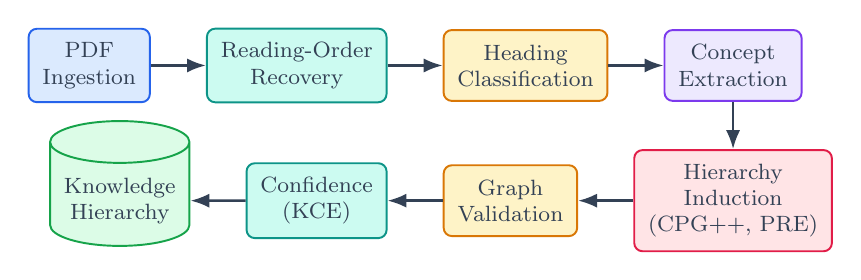
\begin{tikzpicture}[node distance=6mm and 7mm]
\node[stage, sBlue] (a) {PDF\\Ingestion};
\node[stage, sTeal, right=of a] (b) {Reading-Order\\Recovery};
\node[stage, sAmber, right=of b] (c) {Heading\\Classification};
\node[stage, sViolet, right=of c] (d) {Concept\\Extraction};
\node[stage, sRose, below=of d] (e) {Hierarchy\\Induction\\(CPG++, PRE)};
\node[stage, sAmber, left=of e] (f) {Graph\\Validation};
\node[stage, sTeal, left=of f] (g) {Confidence\\(KCE)};
\node[store, left=of g] (h) {Knowledge\\Hierarchy};
\draw[farrow] (a)--(b); \draw[farrow] (b)--(c); \draw[farrow] (c)--(d);
\draw[farrow] (d)--(e); \draw[farrow] (e)--(f); \draw[farrow] (f)--(g); \draw[farrow] (g)--(h);
\end{tikzpicture}
\caption{Processing pipeline from a PDF to a validated concept hierarchy.}
\label{fig:pipeline}
\end{figure}

\section{Data Model}
The representation has two tiers, kept separate so that physical layout is not mixed
with semantic content. Figure~\ref{fig:dualtier} illustrates the two tiers and the link
between them.

Tier~1 stores physical layout: each \textbf{TextBlock} holds its text, page number, font
size, font weight, reading-order rank, and bounding box $(x_0, y_0, x_1, y_1)$ in page points.
Tier~2 stores semantics: each \textbf{ConceptNode} holds a canonical name, an optional
definition, a heading level, a confidence score, and a link to the Tier~1 block it came from.
A \textbf{HierarchyEdge} connects a child concept to its single parent. The hierarchy is a
set of rooted trees (a forest); every non-root node has exactly one parent.

\begin{figure}[!htbp]
\centering
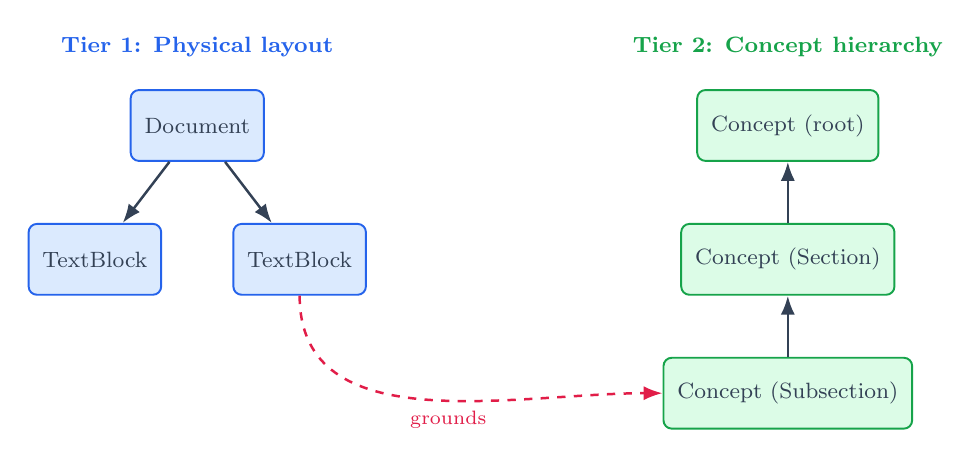
\begin{tikzpicture}[every node/.style={font=\footnotesize}]
% ---- Tier 1: Document -> two TextBlocks placed side by side ----
\node[stage, sBlue] (doc) at (0,0) {Document};
\node[stage, sBlue] (blk1) at (-1.3,-1.7) {TextBlock};
\node[stage, sBlue] (blk2) at ( 1.3,-1.7) {TextBlock};
\draw[farrow] (doc) -- (blk1);
\draw[farrow] (doc) -- (blk2);
\node[text=cBlue] at (0,1.0) {\bfseries Tier 1: Physical layout};
% ---- Tier 2: root -> section -> subsection (vertical chain) ----
\node[stage, sGreen] (root) at (7.5,0) {Concept (root)};
\node[stage, sGreen] (c1) at (7.5,-1.7) {Concept (Section)};
\node[stage, sGreen] (c2) at (7.5,-3.4) {Concept (Subsection)};
\draw[farrow] (c1) -- (root);
\draw[farrow] (c2) -- (c1);
\node[text=cGreen] at (7.5,1.0) {\bfseries Tier 2: Concept hierarchy};
% ---- grounding link from a block to a concept ----
\draw[farrow, dashed, draw=cRose] (blk2.south) to[out=-90,in=180]
      node[below,font=\scriptsize,text=cRose,pos=0.55]{grounds} (c2.west);
\end{tikzpicture}
\caption{Dual-tier data model. Tier~2 concepts are grounded in Tier~1 blocks by an
explicit link to their bounding-box evidence.}
\label{fig:dualtier}
\end{figure}

\section{Layout-Aware Ingestion}
The ingestion step opens the PDF and reads each page's text with position and font
information. For each line it records the bounding box, the most common font size, and
whether the font is bold. The reference implementation uses pdfplumber; any extractor
that reports per-block coordinates and font size (for example, PyMuPDF) can be used in
its place. Scanned or image-only pages would first need OCR, which is outside the scope
of this work.

\section{Reading-Order Recovery}
A PDF does not store text in reading order, and reading a two-column page top-to-bottom
mixes both columns~\cite{huang2022layoutlmv3}. Guided by geometric layout-analysis
principles~\cite{ogorman1993document,breuel2002high}, the system recovers reading order
by splitting the page at the gutter and sorting each column separately.

Let a page have width $W$ and height $H$, and let each block $b$ have a bounding box
$(x_0,y_0,x_1,y_1)$. The algorithm proceeds in three steps.
\begin{enumerate}
  \item \textbf{Spanning blocks.} A block that is wider than $0.60\,W$ spans both
  columns. If it also sits near the top ($y_0 < 0.30\,H$) it is a title or full-width
  header and is placed before the columns; otherwise it is placed after them.
  \item \textbf{Column split.} Remaining blocks go to the left column if $x_1 \le W/2$
  and to the right column otherwise.
  \item \textbf{Within-column order.} Each column is sorted by top coordinate $y_0$.
  Blocks whose tops differ by at most $\tau_y = 20$~pt are treated as one horizontal
  line and ordered left to right by $x_0$.
\end{enumerate}
The final order is: top-spanning blocks, then the whole left column, then the whole
right column, then bottom-spanning blocks. Algorithm~\ref{alg:reading} states the
procedure, and Figure~\ref{fig:reading} contrasts it with naive top-to-bottom reading.

\begin{figure}[!htbp]
\centering
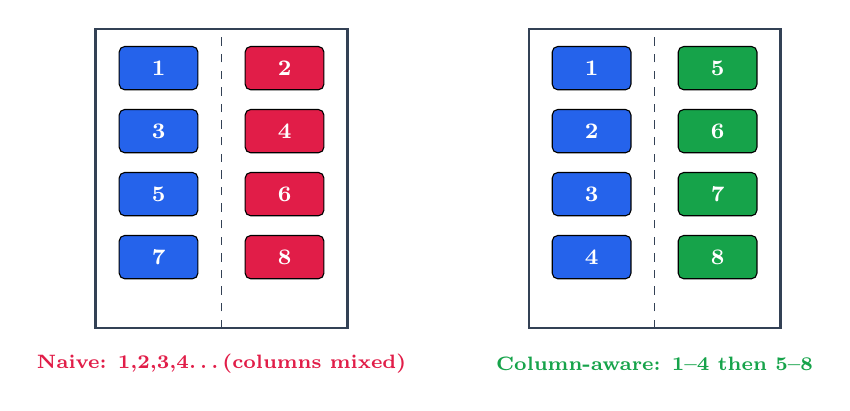
\begin{tikzpicture}[font=\scriptsize\bfseries,
  cell/.style={rounded corners=2pt, minimum width=1.0cm, minimum height=0.55cm,
               draw, text=white, font=\footnotesize\bfseries}]
% naive (columns interleaved) -- order colour goes blue->rose to show scramble
\begin{scope}
  \draw[draw=cSlate, line width=0.8pt] (0,-0.1) rectangle (3.2,3.7);
  \foreach \y/\n in {3.2/1,2.4/3,1.6/5,0.8/7} {\node[cell,fill=cBlue] at (0.8,\y) {\n};}
  \foreach \y/\n in {3.2/2,2.4/4,1.6/6,0.8/8} {\node[cell,fill=cRose] at (2.4,\y) {\n};}
  \draw[dashed,draw=cSlate] (1.6,-0.1)--(1.6,3.7);
  \node[text=cRose] at (1.6,-0.55) {Naive: 1,2,3,4\dots (columns mixed)};
\end{scope}
% gutter (column-first)
\begin{scope}[xshift=5.5cm]
  \draw[draw=cSlate, line width=0.8pt] (0,-0.1) rectangle (3.2,3.7);
  \foreach \y/\n in {3.2/1,2.4/2,1.6/3,0.8/4} {\node[cell,fill=cBlue] at (0.8,\y) {\n};}
  \foreach \y/\n in {3.2/5,2.4/6,1.6/7,0.8/8} {\node[cell,fill=cGreen] at (2.4,\y) {\n};}
  \draw[dashed,draw=cSlate] (1.6,-0.1)--(1.6,3.7);
  \node[text=cGreen] at (1.6,-0.55) {Column-aware: 1--4 then 5--8};
\end{scope}
\end{tikzpicture}
\caption{Naive reading interleaves the two columns; column-aware sorting reads the left
column fully before the right column.}
\label{fig:reading}
\end{figure}

\begin{algorithm}[!htbp]
\caption{Column-Aware 2D Reading-Order Sorting}
\label{alg:reading}
\begin{algorithmic}[1]
\REQUIRE Blocks $\mathcal{B}$ of a page, width $W$, height $H$, tolerance $\tau_y=20$~pt
\ENSURE Ordered blocks $\mathcal{B}_{\text{sorted}}$
\STATE $S_{\text{top}},S_{\text{bot}},C_1,C_2 \leftarrow [\,],[\,],[\,],[\,]$
\FORALL{$b \in \mathcal{B}$}
  \IF{$(b.x_1-b.x_0) > 0.60\,W$ \AND $b.y_0 < 0.30\,H$} \STATE append $b$ to $S_{\text{top}}$
  \ELSIF{$(b.x_1-b.x_0) > 0.60\,W$} \STATE append $b$ to $S_{\text{bot}}$
  \ELSIF{$b.x_1 \le W/2$} \STATE append $b$ to $C_1$
  \ELSE \STATE append $b$ to $C_2$ \ENDIF
\ENDFOR
\FORALL{column $C \in \{C_1,C_2\}$}
  \STATE sort $C$ by $y_0$; group blocks with $|y_{0,i}-y_{0,j}|\le\tau_y$ into a line; order each line by $x_0$
\ENDFOR
\STATE sort $S_{\text{top}},S_{\text{bot}}$ by $y_0$
\RETURN $S_{\text{top}} \oplus C_1 \oplus C_2 \oplus S_{\text{bot}}$
\end{algorithmic}
\end{algorithm}

\section{Heading Classification and Concept Extraction}
The system estimates the body font size as the most common size among long text lines.
A block is treated as a heading if it starts with a section number (matching
\texttt{\^{}\textbackslash d+(\textbackslash.\textbackslash d+)*}) or if its font is at
least $1.25\times$ the body size. For a numbered heading, the level is the count of
number components: ``3'' is level~1, ``3.2'' is level~2, ``3.2.1'' is level~3. For an
unnumbered heading, the level is set from its relative font size. Each heading becomes a
concept node whose name is the heading text and whose evidence link points to the source
block's bounding box. If the first body line after a heading begins with a definitional
cue (``is'', ``are'', ``refers to'', ``is defined as'', ``denotes''), it is stored as
the concept's definition.

\section{Hierarchy Induction}
Each concept must be attached to a parent. Figure~\ref{fig:hier} shows the two-step
procedure: Candidate Parent Generation (CPG++) narrows the candidates, and the Parent
Ranking Engine (PRE) picks one. Both are formulated in this work.

\begin{figure}[!htbp]
\centering
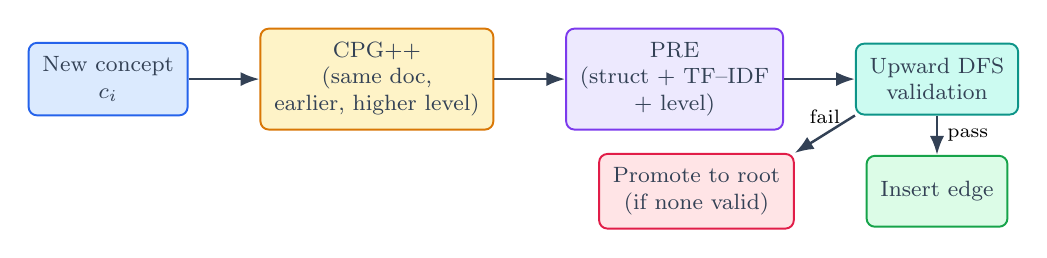
\begin{tikzpicture}[node distance=5mm and 9mm, font=\footnotesize]
\node[stage, sBlue] (n) {New concept\\$c_i$};
\node[stage, sAmber, right=of n] (cpg) {CPG++\\(same doc,\\earlier, higher level)};
\node[stage, sViolet, right=of cpg] (pre) {PRE\\(struct + TF--IDF\\+ level)};
\node[stage, sTeal, right=of pre] (val) {Upward DFS\\validation};
\node[stage, sGreen, below=of val] (ins) {Insert edge};
\node[stage, sRose, left=of ins] (root) {Promote to root\\(if none valid)};
\draw[farrow] (n)--(cpg); \draw[farrow] (cpg)--(pre); \draw[farrow] (pre)--(val);
\draw[farrow] (val)-- node[right,font=\scriptsize]{pass} (ins);
\draw[farrow] (val.south west)-- node[above,font=\scriptsize]{fail} (root.north east);
\end{tikzpicture}
\caption{Hierarchy induction: candidate generation, parent ranking, and validation.}
\label{fig:hier}
\end{figure}

\subsection{Candidate Parent Generation (CPG++)}
For a concept $c_i$, the candidate set contains concepts from the same document that
appear earlier in reading order and have a higher structural level (a smaller level
index):
\begin{equation}
\text{CPG}(c_i)=\{u : \text{doc}(u)=\text{doc}(c_i)\ \wedge\ \text{order}(u)<\text{order}(c_i)\ \wedge\ \text{level}(u)<\text{level}(c_i)\}.
\end{equation}
If this set is empty (for example, when heading levels are ambiguous), the constraint on
level is dropped and any earlier concept in the same document is a candidate. If there
is still no candidate, $c_i$ becomes a root.

\subsection{Parent Ranking Engine (PRE)}
When several candidates exist, PRE scores each candidate $u$ and picks the best:
\begin{equation}
\text{Score}(u,c_i)=w_{\text{struct}}S_{\text{struct}}+w_{\text{sem}}S_{\text{sem}}+w_{\text{level}}S_{\text{level}},
\label{eq:pre}
\end{equation}
with weights $w_{\text{struct}}=0.40$, $w_{\text{sem}}=0.40$, and $w_{\text{level}}=0.20$.
The three terms are each bounded in $[0,1]$:
\begin{itemize}
  \item $S_{\text{struct}}=1/(1+\log(1+\Delta))$, where $\Delta$ is the reading-order
  gap between $u$ and $c_i$; closer candidates score higher.
  \item $S_{\text{sem}}$ is the cosine similarity between the TF--IDF
  vectors~\cite{salton1983introduction} of the two concepts' text; more similar text
  scores higher.
  \item $S_{\text{level}}=\max(0,\,1-0.2(\Delta\mathrm{level}-1))$, which favours an
  immediate parent ($\Delta\mathrm{level}=1$) over a distant ancestor.
\end{itemize}
A dense sentence encoder can replace the TF--IDF term without changing the rest of the
method; TF--IDF is used here because it needs no external model and is fully
reproducible. As the results in Chapter~4 show, section numbering is a stronger signal
than $S_{\text{sem}}$ for numbered documents, so PRE is used mainly for unnumbered
headings.

\section{Structural Validation}
\label{sec:invariants}
Before an edge $(u,c_i)$ is inserted, it is checked against three invariants:
\begin{itemize}
  \item \textbf{Acyclicity.} An upward DFS starts at $u$ and follows parent links. If it
  reaches $c_i$, the edge would create a cycle and is rejected. Because a parent always
  precedes its child in reading order, and the traversal is bounded by the maximum depth,
  this check is inexpensive.
  \item \textbf{Single parent.} A non-root concept keeps exactly one parent.
  \item \textbf{Bounded depth.} No node may exceed depth $D_{\max}=8$.
\end{itemize}
If the chosen edge fails validation, the concept is promoted to a root rather than left
unattached, so there are no orphan nodes. Algorithm~\ref{alg:dfs} states the check.

\begin{algorithm}[!htbp]
\caption{Upward DFS Cycle and Depth Check}
\label{alg:dfs}
\begin{algorithmic}[1]
\REQUIRE candidate edge $(u,v)$ (parent $u$, child $v$), parent map
\ENSURE True if the edge is valid
\IF{$u=v$} \RETURN False \ENDIF
\IF{$\text{depth}(u)+1 > D_{\max}$} \RETURN False \ENDIF
\STATE $stack \leftarrow [u]$, $seen \leftarrow \{v\}$
\WHILE{$stack$ not empty}
  \STATE $x \leftarrow \text{pop}(stack)$
  \IF{$x=v$} \RETURN False \COMMENT{cycle} \ENDIF
  \IF{$x \notin seen$} \STATE add $x$ to $seen$; push $\text{parent}(x)$ if it exists \ENDIF
\ENDWHILE
\RETURN True
\end{algorithmic}
\end{algorithm}

\section{Confidence Estimation}
Each concept gets a confidence score that reflects how clearly it was detected and how
reliable its ancestors are. A local score starts at $0.5$ and adds $0.15$ if the font is
larger than body text, $0.10$ if bold, $0.15$ if it has a section number, and $0.10$ if
a definition was found, capped at $1.0$. Scores are then propagated from roots to leaves
in topological order using Kahn's algorithm~\cite{kahn1962topological}: a child's score
is $C(v)=C_{\text{local}}(v)\,(\delta+(1-\delta)C(\text{parent}))$ with damping
$\delta=0.85$. Processing parents before children keeps the pass deterministic.

\section{Summary}
This chapter described the method: column-aware reading-order recovery, heading-based
concept extraction, hierarchy induction with CPG++ and PRE, upward-DFS validation, and
topological confidence propagation.

% ============================================================================
% CHAPTER 4: WORK DONE
% ============================================================================
\chapter{Work Done}

\section{Implementation}
The system is implemented in Python. Table~\ref{tab:stack} lists the main components.
PDF text and coordinates are read with pdfplumber; TF--IDF similarity uses
scikit-learn; numerical work uses NumPy; and data objects are validated with Pydantic.
The code is organised as six modules that follow the pipeline in Figure~\ref{fig:pipeline}:
ingestion, structural parsing (reading order and heading classification), concept
extraction, hierarchy building (CPG++ and PRE), graph validation, and confidence
scoring.

\begin{table}[!htbp]
\centering
\caption{Implementation components.}
\label{tab:stack}
\renewcommand{\arraystretch}{1.25}
{\small
\begin{tabularx}{\textwidth}{@{} >{\bfseries}l X @{}}
\toprule
Component & Role \\ \midrule
Python 3 & Implementation language \\
pdfplumber & Extract text blocks with bounding boxes and font size \\
scikit-learn & TF--IDF vectors and cosine similarity for the PRE semantic term \\
NumPy & Vector and array operations \\
Pydantic & Validation of Tier~1 and Tier~2 data objects \\ \bottomrule
\end{tabularx}}
\end{table}

\section{Experimental Setup}
The system was evaluated on a corpus of eleven research-paper PDFs in the
retrieval-augmented generation area (for example, TreeRAG, GraphRAG, RAPTOR, Self-RAG,
HiChunk, RETRO, Atlas, T-RAG, REALM, HAT-RAG, and the original RAG paper). These are
digital, mostly two-column academic PDFs, which is the document type this project
targets.

Two things were measured. Reading order was measured by the pairwise inversion rate
against a column-first reference order defined by page geometry (left column top to
bottom, then right column). Hierarchy quality was measured by Parent Assignment
Accuracy (PAA): the fraction of numbered sections whose assigned parent matches the
parent implied by the section numbering (``3.1'' under ``3'').

\section{Reading-Order Results}
Table~\ref{tab:reading} compares naive top-to-bottom extraction with column-aware
sorting. Across the corpus, naive extraction had a mean inversion rate of $21.8\%$
(reading-order monotonicity of $78.2\%$), while column-aware sorting reduced it to
$0.5\%$ (monotonicity of $99.5\%$). Figure~\ref{fig:romchart} shows the per-strategy
means.

\begin{table}[!htbp]
\centering
\caption{Reading-order inversion rate (\%) per document: naive vs.\ column-aware.}
\label{tab:reading}
\renewcommand{\arraystretch}{1.2}
{\small
\begin{tabularx}{\textwidth}{@{} X >{\centering\arraybackslash}p{2.4cm} >{\centering\arraybackslash}p{2.4cm} @{}}
\toprule
Document & Naive inversion (\%) & Column-aware (\%) \\ \midrule
GraphRAG      & 19.1 & 0.1 \\
Atlas         & 18.9 & 0.6 \\
HiChunk       & 23.5 & 0.3 \\
HAT-RAG       & 23.6 & 1.3 \\
RETRO         & 23.1 & 0.4 \\
Self-RAG      & 22.7 & 0.5 \\
RAPTOR        & 20.9 & 0.3 \\
RAG (Lewis)   & 18.6 & 0.4 \\
REALM         & 26.2 & 0.8 \\
T-RAG         & 23.2 & 0.2 \\
TreeRAG       & 20.4 & 0.7 \\ \midrule
\textbf{Mean} & \textbf{21.8} & \textbf{0.5} \\ \bottomrule
\end{tabularx}}
\end{table}

\begin{figure}[!htbp]
\centering
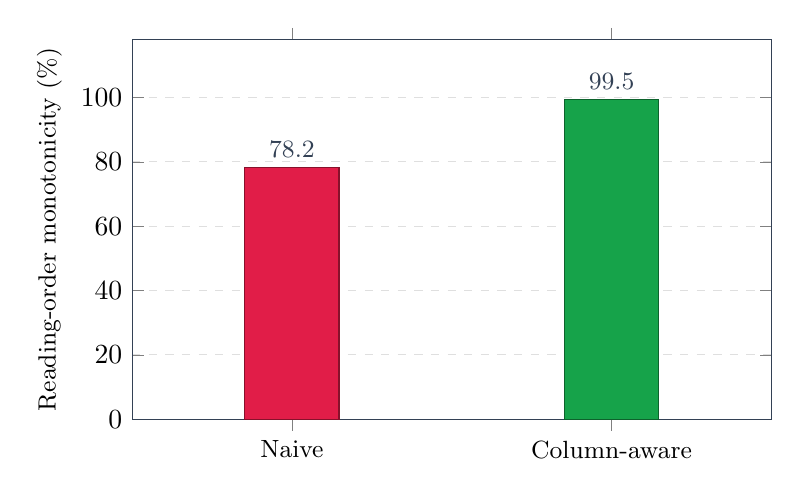
\begin{tikzpicture}
\begin{axis}[ybar, bar width=34pt, bar shift=0pt, width=0.8\textwidth, height=6.4cm,
  enlarge x limits=0.5, ymin=0, ymax=118, ytick={0,20,40,60,80,100},
  clip=false, ylabel={Reading-order monotonicity (\%)},
  ylabel style={font=\small}, symbolic x coords={Naive, Column-aware},
  xtick={Naive,Column-aware}, x tick label style={font=\small}, nodes near coords,
  every node near coord/.append style={font=\small\bfseries, text=cSlate},
  ymajorgrids, grid style={dashed,gray!25}, axis line style={cSlate}]
\addplot[fill=cRose, draw=cRose!60!black] coordinates {(Naive,78.2)};
\addplot[fill=cGreen, draw=cGreen!60!black] coordinates {(Column-aware,99.5)};
\end{axis}
\end{tikzpicture}
\caption{Mean reading-order monotonicity across the eleven-document corpus.}
\label{fig:romchart}
\end{figure}

The gain comes from separating the columns before sorting. Naive extraction interleaves
the columns because blocks at similar heights in different columns are read one after
another. The residual $0.5\%$ comes mostly from full-width figures or tables placed in
the middle of a page, which the gutter rule places after the columns.

\section{Hierarchy Results}
Table~\ref{tab:paa} reports Parent Assignment Accuracy over the $196$ numbered sections
in the corpus, for four attachment methods. Section numbering places every numbered
section under the correct parent. The semantic Parent Ranking Engine, used on its own,
reaches $51.5\%$: it is better than a sequential or lexical rule but clearly weaker than
numbering, because the section number is an almost perfect signal that text similarity
cannot improve on. Figure~\ref{fig:paachart} shows the comparison.

\begin{table}[!htbp]
\centering
\caption{Parent Assignment Accuracy over 196 numbered sections in the corpus.}
\label{tab:paa}
\renewcommand{\arraystretch}{1.25}
{\small
\begin{tabularx}{\textwidth}{@{} X >{\centering\arraybackslash}p{3.0cm} @{}}
\toprule
Attachment method & PAA (\%) \\ \midrule
Sequential (previous heading) & 17.9 \\
Lexical prefix overlap & 34.7 \\
Parent Ranking Engine (TF--IDF semantic) & 51.5 \\
Section numbering (primary signal) & \textbf{100.0} \\ \bottomrule
\end{tabularx}}
\end{table}

\begin{figure}[!htbp]
\centering
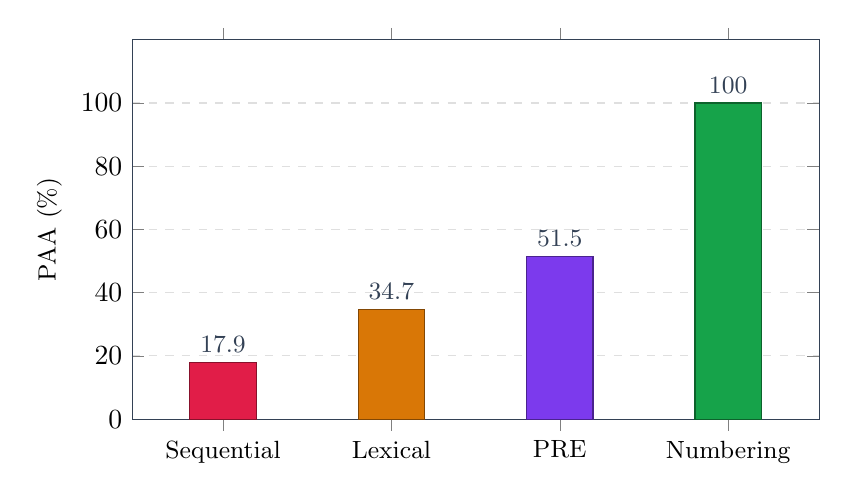
\begin{tikzpicture}
\begin{axis}[ybar, bar width=24pt, bar shift=0pt, width=0.85\textwidth, height=6.4cm,
  enlarge x limits=0.18, ymin=0, ymax=120, ytick={0,20,40,60,80,100},
  clip=false, ylabel={PAA (\%)},
  ylabel style={font=\small}, symbolic x coords={Sequential, Lexical, PRE, Numbering},
  xtick={Sequential,Lexical,PRE,Numbering}, x tick label style={font=\small}, nodes near coords,
  every node near coord/.append style={font=\small\bfseries, text=cSlate},
  ymajorgrids, grid style={dashed,gray!25}, axis line style={cSlate}]
\addplot[fill=cRose,   draw=cRose!60!black]   coordinates {(Sequential,17.9)};
\addplot[fill=cAmber,  draw=cAmber!60!black]  coordinates {(Lexical,34.7)};
\addplot[fill=cViolet, draw=cViolet!60!black] coordinates {(PRE,51.5)};
\addplot[fill=cGreen,  draw=cGreen!60!black]  coordinates {(Numbering,100.0)};
\end{axis}
\end{tikzpicture}
\caption{Parent Assignment Accuracy by method. Numbering is the strongest signal; PRE is
used as a fallback for unnumbered headings.}
\label{fig:paachart}
\end{figure}

This result guided the design: the system uses numbering as the primary signal and calls
the Parent Ranking Engine only for headings that carry no number (for example,
``Abstract'' or ``References''). The combined policy keeps the near-perfect accuracy on
numbered sections while still attaching unnumbered headings sensibly.

Across all eleven documents, the induced hierarchies contained \textbf{no cycles} and
\textbf{no orphan nodes}, and the depth stayed within the bound of eight. These are a
direct result of the validation step in Section~\ref{sec:invariants}: cycles are
rejected by the upward DFS, and any concept that cannot be attached is promoted to a
root instead of being dropped.

\section{Case Study: TreeRAG Paper}
Table~\ref{tab:case} summarises a full run on the 16-page, two-column TreeRAG paper. The
parser extracted 262 text blocks and 15 concept nodes, of which 13 are the paper's
numbered sections. Every numbered section was attached to its correct parent (for
example, ``3.1 Tree-Chunking'' under ``3 TreeRAG'', and ``3.1.1'' under ``3.1''). The
hierarchy had one root, a maximum depth of three, no cycles, and no orphans, and the run
took about 1.8 seconds.

\begin{table}[!htbp]
\centering
\caption{Full run on the TreeRAG paper.}
\label{tab:case}
\renewcommand{\arraystretch}{1.25}
{\small
\begin{tabularx}{\textwidth}{@{} >{\bfseries}l X @{}}
\toprule
Measurement & Value \\ \midrule
Pages & 16 \\
Text blocks extracted & 262 \\
Concept nodes & 15 \\
Numbered sections & 13 (all attached correctly) \\
Hierarchy edges & 14 \\
Maximum depth & 3 \\
Cycles / orphans & 0 / 0 \\
Mean confidence & 0.62 \\
Runtime & $\approx$1.8 s \\ \bottomrule
\end{tabularx}}
\end{table}

\section{Summary}
On the eleven-document corpus, column-aware sorting raised reading-order monotonicity
from $78.2\%$ to $99.5\%$. Section numbering attached $100\%$ of numbered sections
correctly, the Parent Ranking Engine reached $51.5\%$ on its own, and every hierarchy
was acyclic, orphan-free, and within the depth bound.

% ============================================================================
% CHAPTER 5: CONCLUSIONS AND FUTURE WORK
% ============================================================================
\chapter{Conclusions and Future Work}
\vspace{-2mm}

\section{Conclusions}
This project developed a layout-aware parser that converts multi-column PDFs into validated
concept hierarchies. First, column-aware sorting reduced the mean reading-order inversion
rate from $21.8\%$ to $0.5\%$ across eleven research papers. Second, section numbering
proved the most reliable hierarchy signal ($100\%$ accuracy), while the Parent Ranking
Engine served as an effective semantic fallback for unnumbered headings ($51.5\%$ standalone).
Structural validation programmatically ensured acyclicity, zero orphan nodes, and bounded
depth across all evaluated documents.

\section{Limitations}
\begin{enumerate}\setlength{\itemsep}{1pt}\setlength{\parskip}{0pt}\setlength{\parsep}{0pt}
  \item Assumes symmetric two-column layouts split at $W/2$; mid-page full-width floats are not handled ideally.
  \item Evaluated on eleven academic PDFs; non-academic documents may behave differently.
  \item Requires digital text; scanned pages necessitate optical character recognition.
  \item TF--IDF semantic similarity is less effective on heavily paraphrased headings than dense encoders.
  \item Ground truth is based on section numbering, which does not assess unnumbered heading semantics.
\end{enumerate}

\section{Future Work}
\begin{enumerate}\setlength{\itemsep}{1pt}\setlength{\parskip}{0pt}\setlength{\parsep}{0pt}
  \item Replace TF--IDF with a dense sentence encoder for unnumbered headings.
  \item Automatically detect column count and sequence mid-page full-width floats.
  \item Ground generated answers to physical page regions using Tier~1 bounding boxes.
  \item Construct a human-annotated hierarchy to evaluate unnumbered attachments directly.
  \item Test parser generalisation across technical manuals and corporate reports.
\end{enumerate}

% ============================================================================
% REFERENCES
% ============================================================================
\clearpage
\renewcommand{\bibname}{REFERENCES}
\phantomsection
\addcontentsline{toc}{chapter}{REFERENCES}
\begin{thebibliography}{99}

\bibitem{lewis2020rag}
P.~Lewis, E.~Perez, A.~Piktus, et al.
Retrieval-augmented generation for knowledge-intensive NLP tasks.
In \textit{Advances in Neural Information Processing Systems (NeurIPS)}, vol.~33,
pp.~9459--9474, 2020.

\bibitem{guu2020realm}
K.~Guu, K.~Lee, Z.~Tung, P.~Pasupat, and M.~Chang.
REALM: Retrieval-augmented language model pre-training.
In \textit{Proc.\ 37th Int.\ Conf.\ on Machine Learning (ICML)}, pp.~3929--3938, 2020.

\bibitem{borgeaud2022retro}
S.~Borgeaud, A.~Mensch, J.~Hoffmann, et al.
Improving language models by retrieving from trillions of tokens.
In \textit{Proc.\ 39th Int.\ Conf.\ on Machine Learning (ICML)}, pp.~2206--2240, 2022.

\bibitem{izacard2023atlas}
G.~Izacard, P.~Lewis, M.~Lomeli, et al.
Atlas: Few-shot learning with retrieval augmented language models.
\textit{Journal of Machine Learning Research}, 24(251):1--43, 2023.

\bibitem{asai2024selfrag}
A.~Asai, Z.~Wu, Y.~Wang, A.~Sil, and H.~Hajishirzi.
Self-RAG: Learning to retrieve, generate, and critique through self-reflection.
In \textit{Int.\ Conf.\ on Learning Representations (ICLR)}, 2024.

\bibitem{sarthi2024raptor}
P.~Sarthi, S.~Abdullah, A.~Tuli, et al.
RAPTOR: Recursive abstractive processing for tree-organized retrieval.
In \textit{Int.\ Conf.\ on Learning Representations (ICLR)}, 2024.

\bibitem{tao2025treerag}
W.~Tao, X.~Xing, Y.~Chen, L.~Huang, and X.~Xu.
TreeRAG: Unleashing the power of hierarchical storage for enhanced knowledge retrieval
in long documents.
In \textit{Findings of the ACL 2025}, pp.~356--371, 2025.

\bibitem{lu2026hichunk}
W.~Lu, K.~Chen, Z.~Shen, R.~Qiao, and X.~Sun.
HiChunk: Evaluating and enhancing retrieval-augmented generation with hierarchical
chunking.
In \textit{Proc.\ 64th Annual Meeting of the ACL}, pp.~29738--29753, 2026.

\bibitem{fatehkia2024trag}
M.~Fatehkia, J.~Kim Lucas, and S.~Chawla.
T-RAG: Lessons from the LLM trenches.
\textit{arXiv preprint arXiv:2402.07483}, 2024.

\bibitem{edge2024graphrag}
D.~Edge, H.~Trinh, N.~Cheng, et al.
From local to global: A graph RAG approach to query-focused summarization.
\textit{arXiv preprint arXiv:2404.16130}, 2024.

\bibitem{huang2022layoutlmv3}
Y.~Huang, T.~Lv, L.~Cui, Y.~Lu, and F.~Wei.
LayoutLMv3: Pre-training for document AI with unified text and image masking.
In \textit{Proc.\ 30th ACM Int.\ Conf.\ on Multimedia}, pp.~4083--4091, 2022.

\bibitem{ogorman1993document}
L.~O'Gorman.
The document spectrum for page layout analysis.
\textit{IEEE Trans.\ on Pattern Analysis and Machine Intelligence}, 15(11):1162--1173, 1993.

\bibitem{breuel2002high}
T.~M.~Breuel.
Two geometric algorithms for layout analysis.
In \textit{Document Analysis Systems}, pp.~188--199, Springer, 2002.

\bibitem{salton1983introduction}
G.~Salton and M.~J.~McGill.
\textit{Introduction to Modern Information Retrieval}.
McGraw-Hill, 1983.

\bibitem{kahn1962topological}
A.~B.~Kahn.
Topological sorting of large networks.
\textit{Communications of the ACM}, 5(11):558--562, 1962.

\bibitem{tarjan1972depth}
R.~Tarjan.
Depth-first search and linear graph algorithms.
\textit{SIAM Journal on Computing}, 1(2):146--160, 1972.

\bibitem{cormen2009introduction}
T.~H.~Cormen, C.~E.~Leiserson, R.~L.~Rivest, and C.~Stein.
\textit{Introduction to Algorithms}, 3rd ed.
MIT Press, 2009.

\end{thebibliography}

\end{document}
